\documentclass{article}

\usepackage[spanish]{babel}
\usepackage[letterpaper,top=2cm,bottom=2cm,left=3cm,right=3cm,marginparwidth=1.75cm]{geometry}
\usepackage{amsmath}
\usepackage{graphicx}
\usepackage[colorlinks=true, allcolors=darkblue]{hyperref}
\usepackage{parskip}
\usepackage[normalem]{ulem}
\useunder{\uline}{\ul}{}



\title{Tarea 1 - Análisis de Datos I}
\author{Enzo Loiza B.}

\begin{document}

\maketitle

\section*{Pregunta 1}

Se realizó un análisis exploratorio a los siguientes datos de ciudades europeas y americanas:

\begin{table}[h]
\begin{center}
\begin{tabular}{cccccc}
\hline
\textbf{Ciudad} & \textbf{Tamaño} & \textbf{\begin{tabular}[c]{@{}c@{}}Ingreso\\ (USD)\end{tabular}} & \textbf{\begin{tabular}[c]{@{}c@{}}Índice de\\ Criminalidad\end{tabular}} & \textbf{\begin{tabular}[c]{@{}c@{}}Calidad\\ de Aire\end{tabular}} & \textbf{\begin{tabular}[c]{@{}c@{}}Nivel de\\ Desarrollo\end{tabular}} \\ \hline
París & Grande & 60000 & 65 & 6.8 & Alto \\
Zurich & Mediana & 75000 & 30 & 8.0 & Alto \\
Estambul & Grande & 38000 & 58 & 6.7 & Medio \\
Montevideo & Pequeña & 40000 & 30 & 7.0 & Bajo \\
Barcelona & Mediana & 58000 & 35 & 7.5 & Medio \\
Oslo & Mediana & 72000 & 25 & 7.8 & Alto \\
Londres & Grande & 58000 & 30 & 7.0 & Alto \\
Santiago & Grande & 45000 & 38 & 6.3 & Medio 
\end{tabular}
\end{center}
\end{table}

\textbf{a) } En base a los datos, se crearon vectores para cada una de las columnas de manera manual asignando nombres correspondientes (consultar script). Luego, con estos datos, se creó una \texttt{data.frame} con estos vectores:

\begin{verbatim}
df <- data.frame(Ciudad = Ciudad,
                 Tamaño = Tamano,
                 "Ingreso USD" = Ingreso,
                 "Indice Criminalidad" = Criminal_index,
                 "Calidad Aire" = Air_quality,
                 "Nivel Desarrollo" = Development_lvl)
\end{verbatim}

Visualizamos el resultado mediante el comando \texttt{head()}, obteniendo el siguiente resultado:
\begin{verbatim}
      Ciudad  Tamaño Ingreso.USD Indice.Criminalidad Calidad.Aire Nivel.Desarrollo
1      Paris  Grande       60000                  65          6.8             Alto
2     Zurich Mediana       75000                  30          8.0             Alto
3   Estambul  Grande       38000                  58          6.7            Medio
4 Montevideo Pequeña       40000                  30          7.0             Bajo
\end{verbatim}

\textbf{b) } Reportamos las medidas de tendencia central de las variables \texttt{Ingreso.USD}, \texttt{Indice.Criminalidad} y \texttt{Calidad.Aire}, obteniendo los siguientes valores de tendencia central:

\begin{table}[h]
\begin{center}
\begin{tabular}{rccccccc}
\multicolumn{1}{r|}{\textbf{Medida}} & \textbf{Min.} & \textbf{1er Cuartil} & \textbf{Mediana} & \textbf{Moda} & \textbf{Media} & \textbf{3er Cuartil} & \textbf{Max.} \\ \hline
\multicolumn{1}{r|}{\textbf{\begin{tabular}[c]{@{}r@{}}Ingreso\\ (USD)\end{tabular}}}          & 38000         & 43750 & 38000 & 58000 & 55750 & 63000 & 75000 \\
\multicolumn{1}{r|}{\textbf{\begin{tabular}[c]{@{}r@{}}Índice de\\ Criminalidad\end{tabular}}} & 25 & 30 & 32.50 & 30 & 38.88 & 43 & 65 \\
\multicolumn{1}{r|}{\textbf{\begin{tabular}[c]{@{}r@{}}Calidad\\ de Aire\end{tabular}}} & 6.30 & 6.78 & 7.00 & 7.00 & 7.14 & 7.58 & 8.00                   
\end{tabular}
\end{center}
\end{table}

\newpage

Y de dispersión:

\begin{table}[h]
\begin{center}

\begin{tabular}{rcc}
\textbf{Medida} & \textbf{Varianza} & \textbf{Desv. Estándar} \\ \hline
\textbf{\begin{tabular}[c]{@{}r@{}}Ingreso\\ (USD)\end{tabular}} & 191,642,857 & 13,843.51 \\
\textbf{\begin{tabular}[c]{@{}r@{}}Índice de\\ Criminalidad\end{tabular}} & 213.67 & 14.60 \\
\textbf{\begin{tabular}[c]{@{}r@{}}Calidad\\ de Aire\end{tabular}} & 0.34 & 0.58
\end{tabular}
\end{center}
\end{table}

\textbf{c) } Luego, generamos la tabla de frecuencias relativas para las variables \texttt{Tamaño}

\begin{table}[h]
\begin{center}
\begin{tabular}{ccc}
\textbf{Grande} & \textbf{Mediana} & \textbf{Pequeña} \\ \hline
50.00 & 37.50 & 12.50
\end{tabular}
\end{center}
\end{table}


y \texttt{Nivel.Desarrollo}:

\begin{table}[h]
\begin{center}
\begin{tabular}{ccc}
\textbf{Alto} & \textbf{Medio} & \textbf{Bajo} \\ \hline
50.00 & 37.50 & 12.50
\end{tabular}
\end{center}
\end{table}

\section*{Pregunta 2}

\textbf{a) } Realizamos el gráfico de dispersión de ingreso y criminalidad. El código es similar en ambos casos, pues sólo cambiamos la fuente de unos ejes.

\begin{figure}[h!]
    \centering
    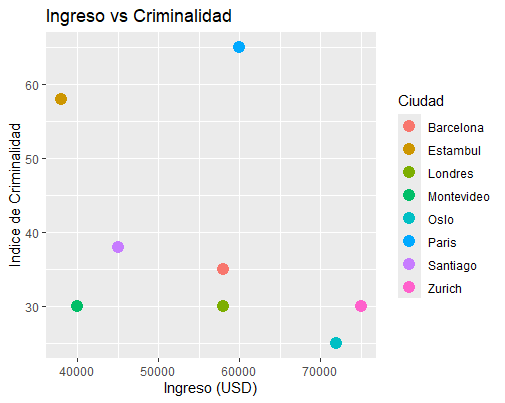
\includegraphics[scale = 0.7]{Tarea_1_2apng.png}
    \caption{Ingreso (USD) versus Índice de Criminalidad}
    \label{fig:enter-label}
\end{figure}

La figura \ref{fig:enter-label}, junto con un \textbf{coeficiente de correlación de -0.36}, indican que existe una correlación negativa moderada entre ambas variables. Esto es, a medida que aumenta el ingreso promedio en una región, tiende a haber una disminución en el índice de criminalidad, y viceversa. Es importante mencionar que esta correlación no indica causalidad, pues aunque puede que existe una influencia de uno sobre otro, puede haber otros factores que no se están considerando en el análisis.

\newpage

\textbf{b) } Realizamos un análisis similar con las variables de Ingreso y Calidad de Aire.

\begin{figure}[h!]
    \centering
    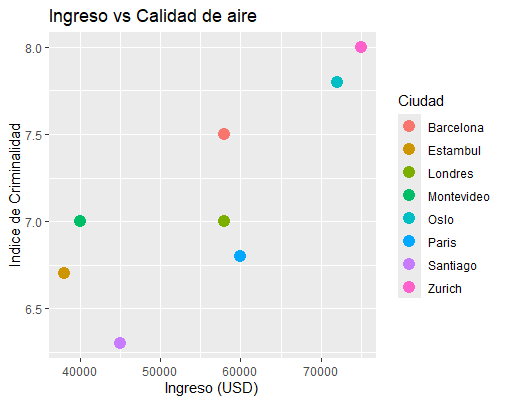
\includegraphics[scale = 0.7]{Tarea_1_2bpng.png}
    \caption{Ingreso (USD) versus Calidad de Aire}
    \label{fig:enter-label2}
\end{figure}

En este caso, en la Figura \ref{fig:enter-label2} se observa una relación fuerte entre el ingreso y la calidad de aire. Esto lo avala un \textbf{coeficiente de correlación de 0.81}, por lo que existe una correlación fuerte positiva entre ambas variables. A medida que aumenta el ingreso de una ciudad, tiende a haber una mejora en la calidad del aire. Sin embargo, al igual que con la correlación entre el ingreso y la criminalidad, es importante considerar varios factores adicionales para comprender completamente la relación\footnote{Compilado en \LaTeX} \footnote{Código disponible en \href{https://github.com/zoendeloi/MPP-ADI}{GitHub}}. 

\end{document}